\section{Túneles GRE}

\subsection{Configuración}
A continuación se detallan las instrucciones de configuraciones de los Routers utilizados para la comunicación hacia Internet.\\
En todos los casos, al configurar el ruteo estático en cada uno de ellos, fuera necesario \textit{pasar por Internet}, la interfaz a la cual se hace referencia será la respectiva al tunel creado. Por ejemplo, se tiene la configuración de ruteo estático de R8 a la red E:
\begin{verbatim}
ip route 10.31.25.0 255.255.255.128 Tunnel20 10.31.25.166 100
\end{verbatim}
Además, debemos indicar cual es el siguiente salto para llegar al destino del tunel, el cual no esta conectado en forma directa a ninguna de las interfaces del router configurado.

\subsubsection{R8}
\begin{verbatim}
interface Ethernet0/2
 description Conexion a INTERNET Q1
 ip address 150.38.27.1 255.255.255.252
 full-duplex

interface Tunnel10 !a R11
 tunnel mode ipip
 ip address 10.31.25.161 255.255.255.252
 tunnel source Ethernet0/2
 tunnel destination 150.38.27.5
!
interface Tunnel20 !a R12
 tunnel mode ipip
 ip address 10.31.25.165 255.255.255.252
 tunnel source Ethernet0/2
 tunnel destination 150.38.27.9
!
\end{verbatim}
Configuración de ruteo necesaria:
\begin{verbatim}
ip route 150.38.27.4 255.255.255.252 150.38.27.2 1
ip route 150.38.27.8 255.255.255.252 150.38.27.2 1
\end{verbatim}


\subsubsection{R11}
\begin{verbatim}
interface Ethernet0/1
 description Conexion a INTERNET Q2
 ip address 150.38.27.5 255.255.255.252
 full-duplex
!
interface Tunnel10 !a R8
 tunnel mode ipip
 ip address 10.31.25.162 255.255.255.252
 tunnel source Ethernet0/1
 tunnel destination 150.38.27.1
!
interface Tunnel30 !a R12
 tunnel mode ipip
 ip address 10.31.25.170 255.255.255.252
 tunnel source Ethernet0/1
 tunnel destination 150.38.27.9
!
\end{verbatim}
Configuración de ruteo necesaria:
\begin{verbatim}
ip route 150.38.27.0 255.255.255.252 150.38.27.6 1
ip route 150.38.27.8 255.255.255.252 150.38.27.6 1
\end{verbatim}

\subsubsection{R12}
\begin{verbatim}
interface Ethernet0/1
 description Conexion a INTERNET Q3
 ip address 150.38.27.9 255.255.255.252
 full-duplex
!

interface Tunnel20 !a R8
 tunnel mode ipip
 ip address 10.31.25.166 255.255.255.252
 tunnel source Ethernet0/1
 tunnel destination 150.38.27.1
!
interface Tunnel30 !a R11
 tunnel mode ipip
 ip address 10.31.25.169 255.255.255.252
 tunnel source Ethernet0/1
 tunnel destination 150.38.27.5
!
\end{verbatim}
Configuración de ruteo necesaria:
\begin{verbatim}
ip route 150.38.27.0 255.255.255.252 150.38.27.10 1
ip route 150.38.27.4 255.255.255.252 150.38.27.10 1
\end{verbatim}

\subsubsection{Internet y Router-Internet}
Para la simulación del servicio de Internet se utilizó un Router C3600, para luego utilizar túneles GRE y permitir el enrutamiento de direcciones privadas, entre distintos routers que se encuentren conectados por medio de Internet. Para realizar la configuración se baso en el apunte de la materia.\\
Para cada conexión hacia Internet (de los Routers antes mencionados), se destinaron 3 subredes de máscara /30, para luego asignar una subred /30 a cada par de conexiones posibles entre los distintos routers.\\
Lo que finalmente se obtiene, es un encapsulamiento de un paquete IP que tiene como destino una dirección privada dentro de otro paquete IP con direccionamiento público, más la existencia de un encabezado GRE. Los routers donde se configura el túnel son los encargados de manipular estos paquetes, armándolos y desarmándolos según corresponda.

La configuración del Router de Internet únicamente consiste en sus interfaces por las cuales se encuentra conectado a los 3 routers mencionados antes. No es necesario (ni debe hacerse) la configuración de ningún tipo de ruteo, puesto que lo único que necesita hacer es mandar los paquetes que recibe hacia routers que se encuentran directamente conectados a él.
\begin{verbatim}
interface Ethernet1/0
 description Conexion INTERNET Q1 con R8
 ip address 150.38.27.2 255.255.255.252
 full-duplex
!
interface Ethernet1/1
 description Conexion INTERNET Q2 con R11
 ip address 150.38.27.6 255.255.255.252
 full-duplex
!
interface Ethernet1/2
 description Conexion INTERNET Q3 con R12
 ip address 150.38.27.10 255.255.255.252
 full-duplex
\end{verbatim}


\begin{figure}
\centering
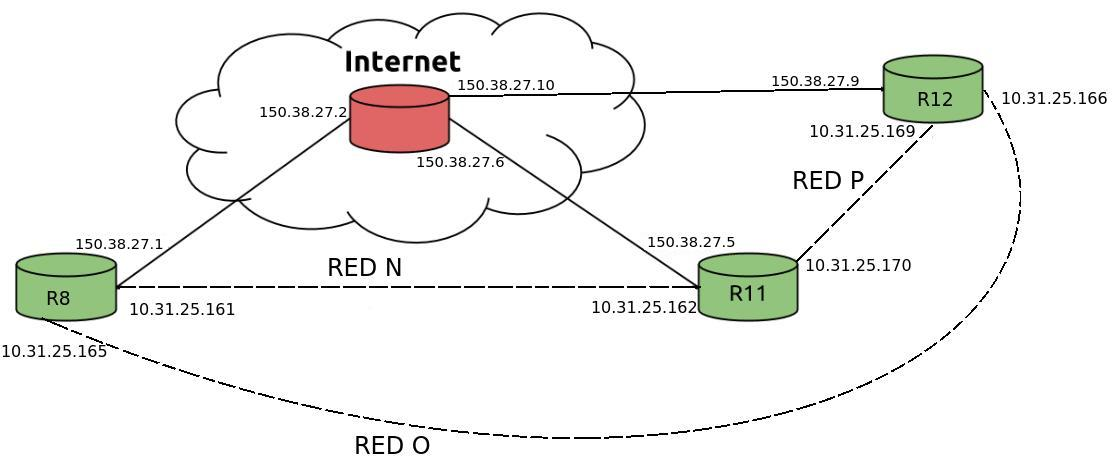
\includegraphics[width=\textwidth]{gre.jpeg} 
\label{gre}
\caption{Esquema de Tunel GRE}
\end{figure}
